\section{Extraction of the G Double-Polarization Observable}
The cross section for this reaction, considering the target linear Polarization along the photon beam direction $P_z$, and the Polarization of the photon beam (PARA, $P_{\parallel}$ (Electric field parallel to the floor) and PERP, $P_{\perp}$ (Electric field perpendicular to the floor)), can be written as:
\begin{equation}
  \frac{d\sigma}{d\Omega} = \left(\frac{d\sigma}{d\Omega}\right)_{UNPOL}  \left( 1 + P_{\gamma}\Sigma cos(2\phi) + P_{\gamma} P_z G sin(2\phi) \right)
  \label{eqn:extract_G_S}
\end{equation}

During the g9a run period all the possible combinations of different polarizations were measured:

\begin{eqnarray}
\left(\frac{d\sigma}{d\Omega}\right)_{\parallel +} = \left(\frac{d\sigma}{d\Omega}\right)_{UNPOL}  \left( 1 + P_{\gamma \parallel}\Sigma cos(2\phi) + P_{\gamma \parallel} P_{+z\parallel} G sin(2\phi) \right) \\
\left(\frac{d\sigma}{d\Omega}\right)_{\parallel -} = \left(\frac{d\sigma}{d\Omega}\right)_{UNPOL}  \left( 1 + P_{\gamma \parallel}\Sigma cos(2\phi) - P_{\gamma \parallel} P_{-z\parallel} G sin(2\phi) \right) \\
\left(\frac{d\sigma}{d\Omega}\right)_{\perp +} = \left(\frac{d\sigma}{d\Omega}\right)_{UNPOL}  \left( 1 - P_{\gamma \perp}\Sigma cos(2\phi) - P_{\gamma \perp} P_{+z\perp} G sin(2\phi) \right) \\
\left(\frac{d\sigma}{d\Omega}\right)_{\perp -} = \left(\frac{d\sigma}{d\Omega}\right)_{UNPOL}  \left( 1 - P_{\gamma \perp}\Sigma cos(2\phi) + P_{\gamma \perp} P_{-z\perp} G sin(2\phi) \right)
\end{eqnarray}
The construction of asymmetry observables between these combinations allows the simulatneus extraction of G and $\Sigma$ (see chapter \ref{ch:extract_G_S}). In order to normalize these measurement data with an unpolarised photon beam was also obtained in the FROST run period using an amorphous (AMO) crystal (carbon) (See next chapter \ref{ch:flux}). 

\subsection{Calculation of the flux on target, F} \label{ch:flux}
During the experiment, every effort was made to collect the same amount of data for all four possible combinations of (polarised beam)-(polarised target) settings. In practice, however, the flux incident on the target for the PARA and PERP beam settings was not equal and the $\pi^+$ azimuthal distributions (See Fig. \ref{fig:frost_PARA_ex} for an example) had to be scaled to each other before any further analysis.
\begin{figure}[htb]
  \begin{center}
    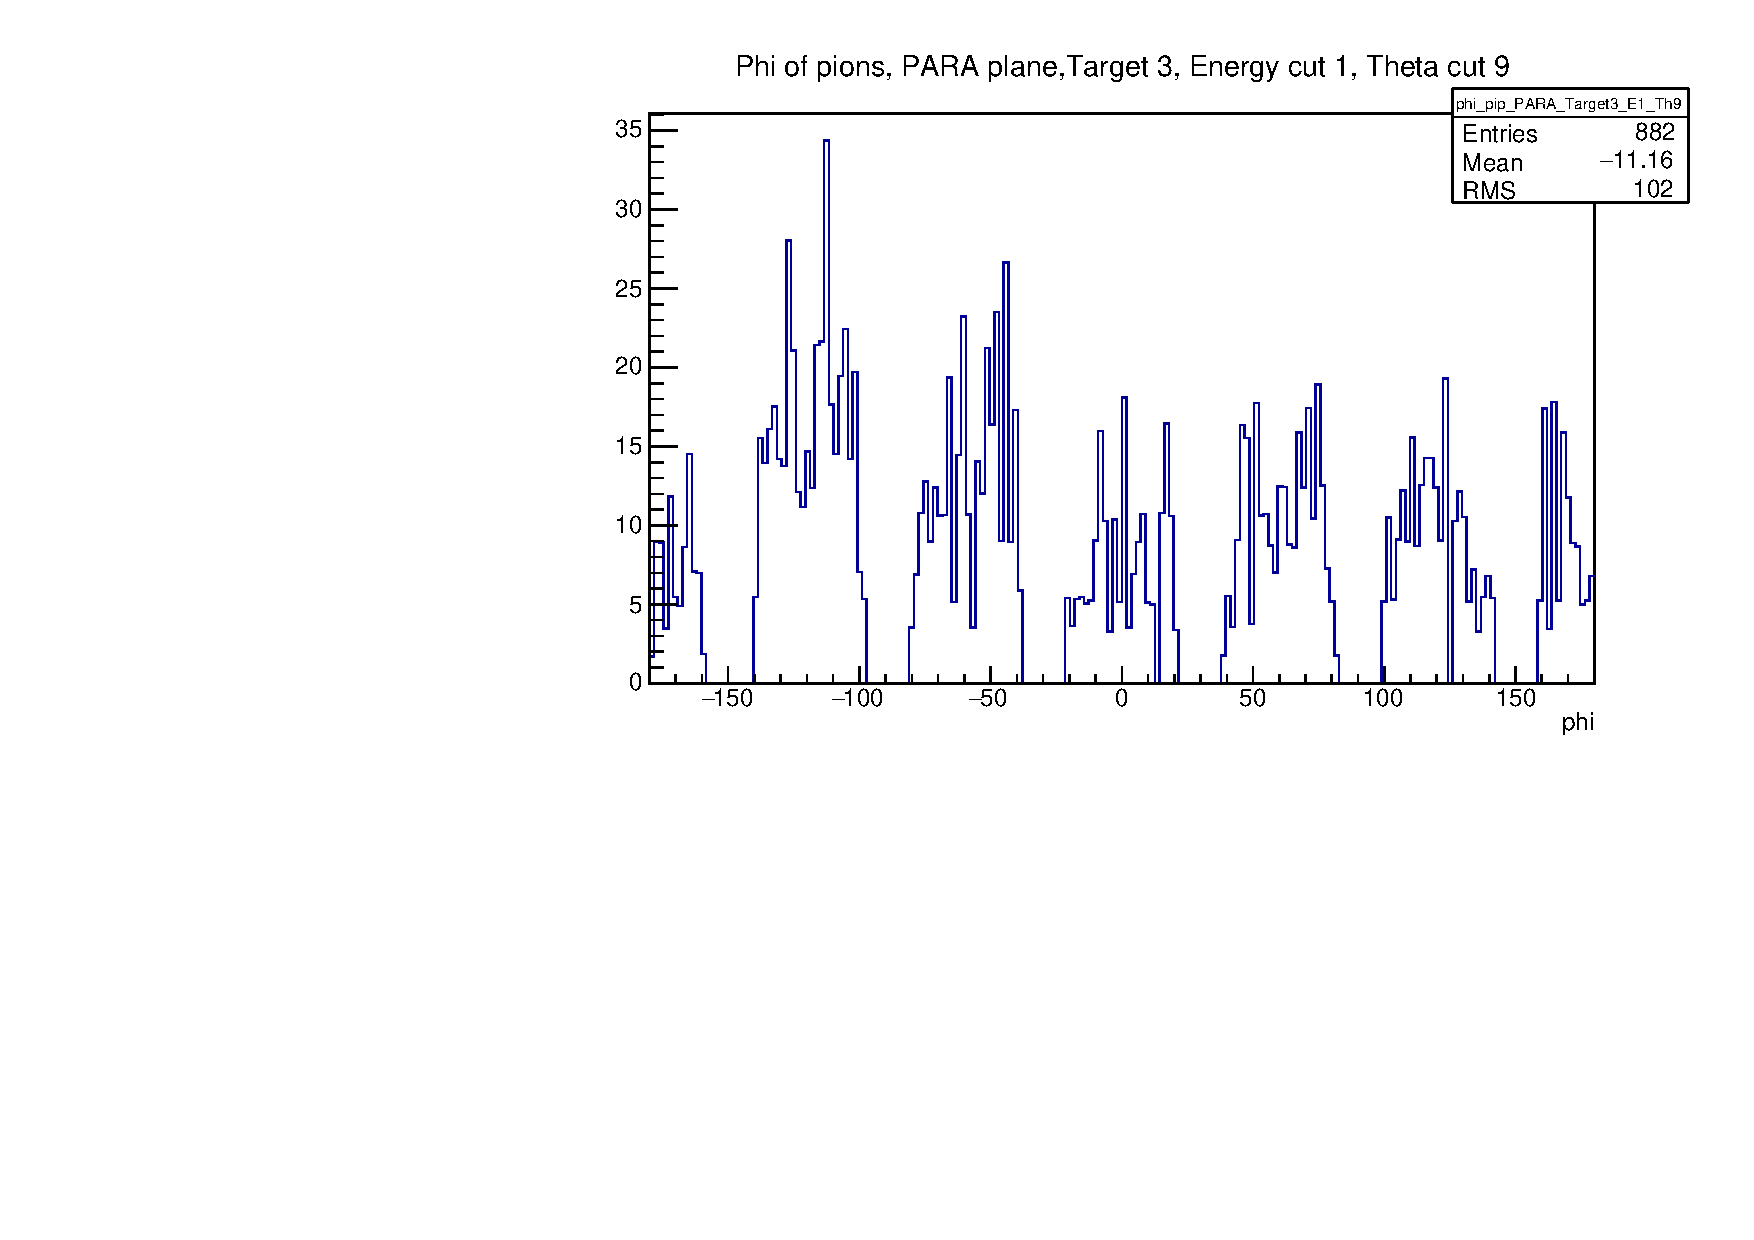
\includegraphics[width=0.6\textwidth]{figures/phi_PARA.pdf} \\
    \caption{$\phi$ distribution for PARA events for a single energy bin and $cos(\theta_{CM})$ bin. }
    \label{fig:frost_PARA_ex}
  \end{center}
\end{figure}



The PARA and PERP $\pi^+$ distributions for a particular target setting were first divided through by the AMO data to remove acceptance effects.
Considering now as:
\begin{enumerate}
  \item $F$ is the flux on target for each beam setting, which is dependent on both energy and linear beam polarisation. 
  \item $\phi_0$ is the “phi-offset” which accounts for any small misalignment of the diamond resulting in the beam polarisations not being exactly parallel or exactly perpendicular to the floor.
\end{enumerate}

\begin{eqnarray}
N_{\parallel +} = \frac{F_{\parallel}}{F_{AMO}} \left( 1 + P_{\gamma \parallel}\Sigma cos(2(\phi-\phi_0)) + P_{\gamma \parallel} P_{+z\parallel} G sin(2(\phi-\phi_0)) \right) \label{eq:N1}\\
N_{\parallel -} = \frac{F_{\parallel}}{F_{AMO}} \left( 1 + P_{\gamma \parallel}\Sigma cos(2(\phi-\phi_0)) - P_{\gamma \parallel} P_{-z\parallel} G sin(2(\phi-\phi_0)) \right) \label{eq:N2}\\
N_{\perp +} = \frac{F_{\perp}}{F_{AMO}} \left( 1 - P_{\gamma \perp}\Sigma cos(2(\phi-\phi_0)) - P_{\gamma \perp} P_{+z\perp} G sin(2(\phi-\phi_0)) \right) \label{eq:N3}\\
N_{\perp -} = \frac{F_{\perp}}{F_{AMO}} \left( 1 - P_{\gamma \perp}\Sigma cos(2(\phi-\phi_0)) + P_{\gamma \perp} P_{-z\perp} G sin(2(\phi-\phi_0)) \right) \label{eq:N4}\\
\end{eqnarray}


These distributions where fitted with a function with 4 parameters ($ a,b,c,d $) :
\begin{equation} \label{eqn:fit_flux}
f(\phi) = a \{ 1 + b\, cos[2 (\phi - c) ]  + d\, sin[2(\phi - c)] \} 
\end{equation}
In this fit, $a$ will be directly related to the value that will be use to normalize the PERP and PARA fluxes and $c$ will be a check of the possible $\phi_0$ offset for possible diamond misalignement.
This method of dividing by the amorphous data before forming an asymmetry was necessary to allow the PARA and PERP flux to be extracted separately. In order to take care of possible fluctuations, this calculation was performed for each energy bin. The fit was optimized by calculating first $\phi_0$ and then fixing this value in the fit. 
Using the results of the fits for the PARA ($\parallel$) and PERP ($\perp$) configurations, the ratio between the two different measurements can be determined (using eqn. \ref{eqn:fit_flux}) as:
\begin{equation}
\frac{F_{\perp}}{F_{\parallel}} = \frac{a_{\perp}}{a_{\parallel}}
\end{equation}

\subsection{Calculation of the Dilution Factor}
\label{ch:dil_factor}
The dilution factor (see equation \ref{eqn:dil_factor}) was calculated for each energy and $cos(\theta_{CM})$ bin using data obtained from the carbon target to model the unpolarised nucleon background in the butanol target.
As the four vectors of the incident photon, target proton and outgoing pion were known, the neutron four-vector was reconstructed using the missing mass technique:
$$
\gamma \, + \,  p \, \rightarrow \, \pi^+ \, + \, X
$$
\begin{figure}[htb]
  \begin{center}
    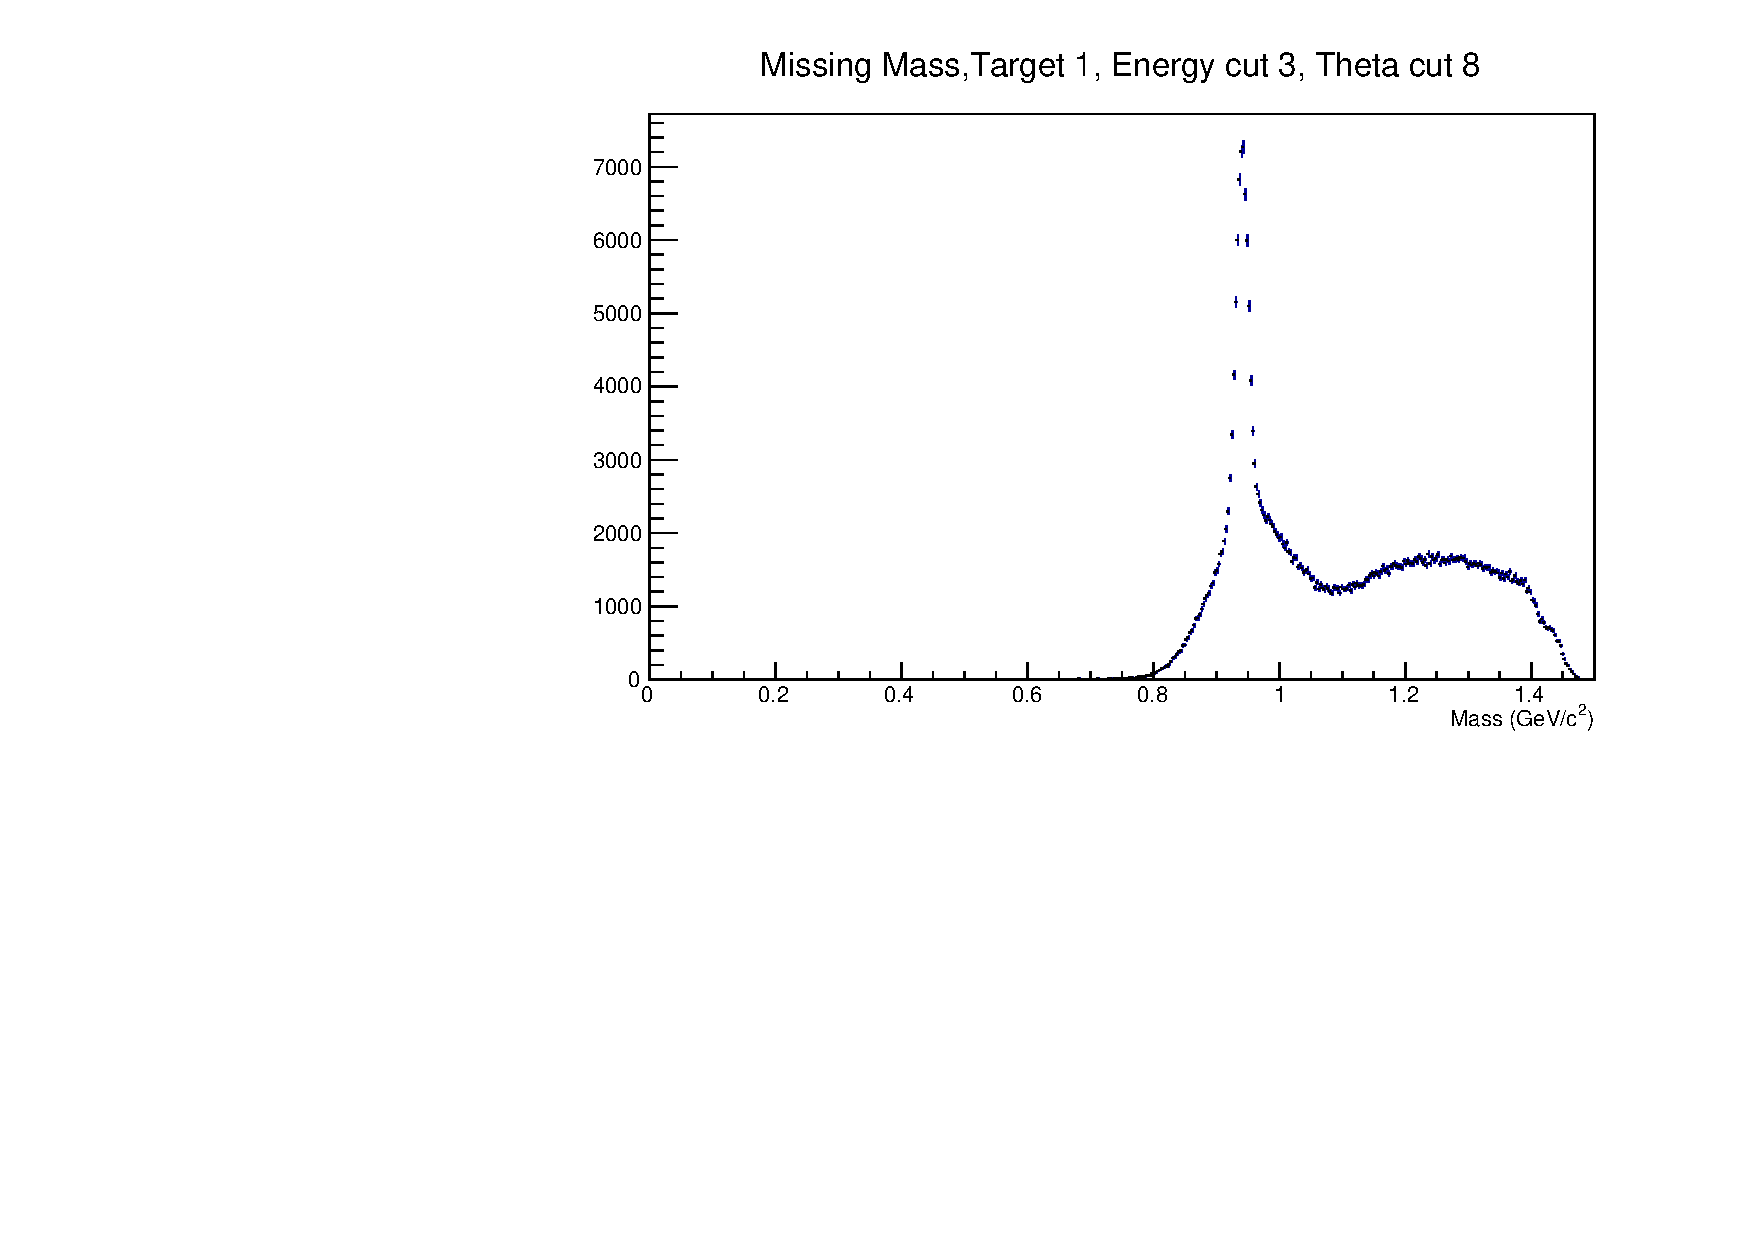
\includegraphics[width=0.6\textwidth]{figures/neutron_missingmass.pdf} \\
    \caption{Mass distribution obtained from the reconstructed neutron four-vector, displaying a sharp peak corresponding to the reconstructed neutron and
a broad peak to the right of this corresponding mainly to two-pion production channels. }
    \label{fig:frost_neutronmissing_ex}
  \end{center}
\end{figure}
\begin{figure}[htb]
  \begin{center}
    \includegraphics[width=0.6\textwidth]{figures/scaling_dilutionfactor.pdf} \\
    \caption{Fitting of the ratio of butanol missing mass distribution with carbon missing mass distribution. The function used is a Gaussian plus a zeroth order polynomial: The zeroth order polynomial will give the constant scaling factor for the carbon target missing mass distribution. }
    \label{fig:scaling_dilutionfactor}
  \end{center}
\end{figure}
assuming momentum is conserved in this reaction. Here X can represent the neutron, other neutral particles, or combinations of positively and negatively charged particles such as $\pi^+ , \pi^-$. Fig. \ref{fig:frost_neutronmissing_ex} shows an example of the missing mass distribution obtained from the reconstructed n four-vector in the butanol target, showing a sharp peak corresponding to the missing neutron mass and a broad peak to the right of this corresponding to other possible channels such as multi-pion production. This plot also shows background contributions due to photon interactions with the carbon and oxygen atoms in the butanol target.
A mass cut was performed to select the neutron and hence the $\pi + n$ events of interest: Following the systematic study on the neutron width done by S. Strauch in \cite{Strauch_2014} a cut of $2 \sigma$ around the neutron missing mass was used in each bin. The width of the neutron-mass cut was determined by making a rough subtraction of the carbon and oxygen background using the missing mass distribution obtained from the carbon target data. The missing-mass distribution obtained from the carbon target was first scaled to the butanol missing-mass distribution. To obtain the scale factor, the butanol missing mass spectrum was divided by the carbon missing mass spectrum and fit with a Gaussian function and a zeroth order polynomial in the region to the left and right of this peak (as shown in Fig. \ref{fig:scaling_dilutionfactor}). 
As the carbon and butanol targets were very close together in the beamline and could not be fully resolved in the z-vertex distribution spectrum, some events within the carbon z-vertex cuts will have originated from polarised protons within the butanol target. Another issue was ice formed in the face of the carbon farther from the butanol target (see Fig. \ref{fig:dilution_factor_z0}). For this last problem, the missing mass distribution was plotted versus the vertex reconstructed with the MVRT bank. A dependence was found with a strong hydrogen contamination for the face of the carbon target farther from the butanol (see Fig. \ref{fig:dilution_factor_z0}). A cut was applied to the MVRT.Z position for each beam configuration in order to remove the part of the spectrum that showed a strong hydrogen contamination (See Table \ref{table:dil_factor_zcut}): This approach was seen as more consistent for all different bins and settings than a double fitting procedure for removing the main part of the hydrogen contamination. In order to remove the remaining part of this contamination, a final fit was done on the carbon missing mass distribution using a combination of a Gaussian function and a third order polynomial. The Gaussian function represented the neutron peak due to the photon interaction with the carbon and oxygen nuclei. Neutron events originating from the photon interaction with a carbon or oxygen nucleus in butanol would be expected to form a peak similar in shape to the neutron peak corresponding to events from the hydrogen atom, but broadened due to the Fermi motion of the nucleons in the carbon or oxygen nucleus. The polynomial modeled the broad background coming from mostly multi-pion production and other non-quasi-free processes. In order to remove the possibility of the fit to model the remaining part of the hydrogen contamination a lower limit was set for the $\sigma$ of the Gaussian function, using the value for the same parameter obtained from the butanol target (See Fig. \ref{fig:dilution_mass_zcut}). The integral of the butanol spectrum and the carbon function within the neutron mass cuts were then obtained, allowing the dilution factor to be calculated as:
\begin{equation} \label{eqn:dil_factor}
  f = \frac{N_B - N_C}{N_B}
\end{equation}
The error on the butanol spectrum was calculated using directly the derived error from the Integral calculation. In order to have a safer approach in determining the carbon fitted error, it was used the area shaped by the sum of the errors of each statistical point in the range defined by the neutron cut (See Fig. \ref{fig:dilution_fit_comp}). 
\begin{figure}[htb]
  \begin{center}
    \subfloat[][Carbon missing mass spectrum (X(GeV)) vs MVRT.Z position (Y(cm))] {
      \includegraphics[width=0.64\textwidth]{figures/mvrt_cut_dilution_factor_1_1.pdf} 
      \label{fig:dilution_factor_z1}
    }
    \qquad
    \subfloat[][Carbon missing mass spectrum in GeV for 5.7cm $<$ MVRT.Z $<$ 6.2cm] {
      \includegraphics[width=0.32\textwidth]{figures/mvrt_cut_dilution_factor_1.pdf}
    \label{fig:dilution_factor_z2}
    }
    \qquad
    \subfloat[][Carbon missing mass spectrum in GeV for 6.8cm $<$ MVRT.Z $<$ 7.3cm] {
      \includegraphics[width=0.32\textwidth]{figures/mvrt_cut_dilution_factor_2.pdf}
    \label{fig:dilution_factor_z3}
    } 

    \caption{The missing mass spectrum is plotted for the carbon target as a function of the reconstructed vertex from the MVRT bank. The spectrum is expected to be independent of the reconstructed Z, but a strong hydrogen contamination is shown for higher Z values. The added Hydrogen spectrum as shown in Fig. \ref{fig:dilution_factor_z3} is compared and consistent with the butanol hydrogen spectrum for the same angle and energy range. Subtracting the hydrogen contamination peak from the carbon will be strongly dependent on the statistic in the bin and on the difference in the shape of background and contamination. A safer approach has been used applying a Z cut to just consider the part of the missing mass spectrum that does not show strong hydrogen contamination. A second fit is then applied to this sample (See Fig. \ref{fig:dilution_mass_zcut}) In order to remove the last part of the hydrogen contamination (probably mainly due to poor vertex reconstruction).}
    \label{fig:dilution_factor_z0}
  \end{center}
\end{figure}

\begin{table}
  \begin{center}
    \begin{tabular}{ ||l|r|r|r|r|r|r|r|r|r||}
      \hline
      \multicolumn{10}{|c|}{g9a Run period: Linearly polarized } \\
      \hline
      $Coh_{Edge}$(GeV)&0.73&0.93&1.1&1.3&1.5&1.7&1.9&2.1&2.3 \\
      \hline
      $Z_{cut}$(cm)&6.1&6.1&6.2&6.2&6.2&6.4&6.4&6.4&6.5 \\
      \hline
    \end{tabular}
  \end{center}
  \caption{g9a Run period: Different Energies for the Coherent Edge Polarization ($Coh_{Edge}$) are shown together with the MVRT.Z upper limit used in order to avoid the area where it appear an hydrogen contamination (probably ice). See Fig. \ref{fig:dilution_factor_z0}.}
  \label{table:dil_factor_zcut}
\end{table}

\begin{figure}[htb]
  \begin{center}
    \includegraphics[width=0.8\textwidth]{figures/plot_dil_730_tot_E1_theta6.png} \\
    \caption{Missing Mass distribution for the carbon target before (BLUE) and after(RED) the Z cut (The histogram after the Cut is scaled to the one before the cut in order to compare the spectrums). A fitted function is used to smooth the carbon missing mass distribution (a Gaussian plus a polynomial of 3-rd order): This last fit will get rid of possible last hydrogen contamination in the spectrum. For the error on the carbon subtraction, I have used the area delimitated by the statistical error of each bin in the carbon histogram in the range where the butanol missing mass is considered (in this bin the $-2\sigma - 2\sigma$ range includes values from 0.91GeV to 0.97GeV).}
    \label{fig:dilution_mass_zcut}
  \end{center}
\end{figure}


\begin{figure}[htb]
  \begin{center}
    \subfloat[][Energy Cut 1] {
      \includegraphics[width=0.25\textwidth]{figures/plot_dil_1300_tot_E0_theta6.png} 
      \label{fig:dilution_comp_E0}
    }
    \subfloat[][Energy Cut 2] {
      \includegraphics[width=0.25\textwidth]{figures/plot_dil_1300_tot_E1_theta6.png}
    \label{fig:dilution_comp_E1}
    }
    \subfloat[][Energy Cut 3] {
      \includegraphics[width=0.25\textwidth]{figures/plot_dil_1300_tot_E2_theta6.png}
    \label{fig:dilution_comp_E2}
    }
    \subfloat[][Energy Cut 4] {
      \includegraphics[width=0.25\textwidth]{figures/plot_dil_1300_tot_E3_theta6.png}
    \label{fig:dilution_comp_E3}
    } \\
    \subfloat[][Dilution factor vs W for  $ 0.2 <= cos(\theta_{CM})<0.4$] {
      \includegraphics[width=0.5\textwidth]{figures/comp_DF_TGPOL_system_6.png}
      \label{fig:dilution_fit_theta6}
      }
    \subfloat[][Comparison of fitted carbon Missing mass distribution] {
      \includegraphics[width=0.5\textwidth]{figures/dilution_factor_1300_E1_E2_theta6_comp2.pdf}
      \label{fig:dilution_fit_comp2}
      }
    \caption{Missing Mass distribution for butanol (BLUE) and carbon(RED) after the Z cut for the carbon target. A fitted function (RED line)  is used to smooth the carbon missing mass distribution (a Gaussian plus a polynomial of 3-rd order). This bin corresponds to the Coherent edge of 1.3GeV (This data-set has been divided into 4 W bins; For this settings, the contribution for butanol in the missing mass spectrum (and so for the dilution factor) is considered just in the range from $\sim 0.88$ GeV to $\sim 0.99$ GeV). The W dependence for this data set (see Fig. \ref{fig:dilution_fit_theta6} and Fig. \ref{fig:dilution_comp_E0},\ref{fig:dilution_comp_E1},\ref{fig:dilution_comp_E2},\ref{fig:dilution_comp_E3} for each Energy-bin distribution contributing to this plot) shows a strong difference between the first energy bin and the other energy bins. The reason for the difference is due to an underlying structure in the hydrogen and carbon spectrum in this energy range (see Fig. \ref{fig:comparison_dilutionfactor}). In order to show the reason for defining the carbon error, in Fig. \ref{fig:dilution_fit_comp2} it is plotted the scaled carbon fitted function for the next energy bin. One can see how the fitting is somehow overcounting for one bin and be undercounting for the next. For this reason as error for the carbon subtraction I have kept the area defined by the error in the carbon data histograms (in the $2\sigma$ missing mass range). \\
      From $W\geq 1.8 GeV$ it is not expected a strong W dependence in the dilution factor. For this reason a final fit is applied to the dilution factor as a function of W for different angle ranges (in the CM) (See Fig. \ref{fig:dilution_fit_theta6}): Different functions have been used for different $e^-$ beam energy, since this will affect directly the photon resolution and so directly the width of the neutron peak. The final value for the dilution factor in this range will be the value of this final fit. In order to keep a conservative approach, for the error on the dilution factor for each bin I have kept the error at each point. }
    \label{fig:dilution_fit_comp}
  \end{center}
\end{figure}

The Dilution factor still showed some structure for $W < 1.8GeV$, especially for $\theta_{CM}$ not in the forward or backward production region. The same structure was seen also in the previous analysis by S. Strauch in \cite{Strauch_2014} that used circularly polarized photon beam (Keeping into consideration that in this previous analysis, with a better photon resolution due to lower electron energy, the dilution factor was higher than the one calculated here). This is directly related to the W dependence of the $\pi^+$ photoproduction from the proton, as shown in Fig. \ref{fig:comparison_dilutionfactor}. For $W \geq 1.8GeV$ the Dilution factor it is not expected to show any structure: For this reason, a linear fit was used to smooth fluctuations, but the error of every single measurement for the dilution factor was kept. A full picture of the dilution factor for each $cos(\theta_{CM})$ bin is shown in the appendix \ref{app:dilfactor} from page \pageref{app:dilfactor}.  

\begin{figure}[htb]
  \begin{center}
    \includegraphics[width=0.6\textwidth]{figures/comp_DF_maid_crosssection.pdf} \\
    \caption{Dilution factor for a single $cos(\theta_{CM})$ bin vs W (RED, GREEN, BLUE points correspond to different electron beam energy settings). Here is plotted together with the scaled total cross section for $\pi^+$ photoproduction on proton from the MAID 2007 model \cite{MAID_2007} (BLACK points). Since for $W \geq 1.8GeV$ it is not expected a fluctuation on the Dilution factor, a linear fit is used for the two electron beam energy settings in this range in order to mitigate possible fluctuations in the extraction of G.}
    \label{fig:comparison_dilutionfactor}
  \end{center}
\end{figure}


\subsection{Calculation of Systematic Corrections from the extraction of G and \texorpdfstring{$\Sigma$}{Sigma}}
\label{ch:sys_corr}
Simulating the construction and extraction of G and $\Sigma$ was important in addressing where to improve the analysis and to quantify systematic correction induced by the process of extraction on real data. Different tests have been done in order to address different methods of filling histograms and how different distributions of the parameters involved could affect the extraction of G and $\Sigma$. Based on equation \ref{eqn:extract_G_S} different distributions and values have been tested:
\begin{enumerate}
\item Photon Polarization ($P_{\gamma}$) was tested for:
  \begin{enumerate}
  \item different shape at each bin with different RMS,
  \item double peak (when two different run periods have the same configuration),
  \item a random error distributed as Gaussian.
  \end{enumerate}
\item Target Polarization ($P_z$)  was tested for
  \begin{enumerate}
  \item different shape at each bin with different RMS,
  \item double peak (when two different run periods have the same configuration)
  \end{enumerate}
\item Since the extraction of G and $\Sigma$ is correlated a grid for both values was tested
\item Different statistics for Parallel and Perpendicular photon polarization settings
\item Two different ways of filling the $\phi$ distributions have been tested:
  \begin{enumerate}
  \item Filling the histograms without any weighting
  \item Filling the histograms with a weight of $(1/P_{\gamma})$ in order to try to normalize the weight of different events with different Photon polarization  $P_{\gamma}$.
  \end{enumerate}
\end{enumerate}
Analyzing the results of these simulations (see Appendix \ref{app:simcode} for a sample of the code used) gave some interesting insights on how to address the analysis of the data.
\subsubsection{Photon Polarization}
For the photon polarization, different shapes and RMS have been tested. No dependence has been seen while using weighted histograms (see section \ref{sec:weighthisto}) with different shapes and RMS for different statistics. The important part was getting the correct mean value for the Beam polarization. For this reason, the statistical error induced in integrating different values of beam polarization in a single observation bin (in $W$ and $cos(\theta_{CM})$ ) was given by the error in obtaining the mean of the Beam Polarization. A systematic error of 10\% was added as a systematic error in the extraction of the Beam Polarization
\subsubsection{Target Polarization}
Target polarization is slowly varying through the experimental data taking. There is so no strong dependence for the same observation bin (see appendix at section \ref{app:tgpol}). If more than a single data period was used in the same configuration, two different target polarization will appear. This will cause the fitting procedure to fail, giving close to zero values for G and wrong values for $\Sigma$. For this reason, observation bins, where two distinct target polarizations were observed, were treated separately.   
\subsubsection{Correction for different calculated G and \texorpdfstring{$\Sigma$}{Sigma} and different statistics}
The extraction of G and $\Sigma$ from the data is highly correlated and simulation showed that there is a dependence on the number of events in each observation bin. For this reason, these 3 variables (G, $\Sigma$, $N_{ev}$) were investigated with multiple simulations that covered their full range. A systematic shift was seen for the extracted values of G and $\Sigma$ for observation bin with statistics below 5000 events. In this region, and in the full range of G and $\Sigma$, multiple simulations (100 simulations) were done with the same settings (G,$\Sigma$, number of events) in order to mitigate statistical fluctuations and establishing a set of Systematic corrections. The averaged systematic correction was then plotted for the same number of events as a function of the calculated G and calculated $\Sigma$ (see Fig. \ref{fig:sys_correction_100} for an example). The reason to plot it as a function of calculated values was done in order to simplify the evaluation of the systematic correction on real data. For each calculated value of G and $\Sigma$, an interpolated value was determined for the systematic correction and for the systematic correction error at each number of events available (See Fig. \ref{fig:calc_sys_correction}). A final interpolation was done in order to extract the systematic correction for the correct $N_{ev}$ in the experimental bin. \\
A full picture of the systematic correction for G and $\Sigma$ obtained from the simulation is shown in the appendix (see chapters \ref{app:G_syscorr} and \ref{app:Sigma_syscorr}). It is interesting to see how the correction changes sign and increase at high speed when the statistic of the events goes below a certain threshold. It is important for this reason to keep the statistic in each observation bin over this threshold.
\begin{table}
  \begin{center}
    \begin{tabular}{ ||c|c|c|c|c|c|c|c|c|c|c|c|c|c||}
      \hline
      \multicolumn{14}{|c|}{Number of Events ($N_{ev}$) simulated for the full G (11 points) and $\Sigma$ range (11 points)  } \\
      \hline
      \hline
      50&60&70&80&90&100&110&120&130&140&150&160&170&180\\
      \hline
      190&200&250&300&350&400&500&600&700&800&900&1000&2000&3000 \\
      \hline
    \end{tabular}
  \end{center}
  \caption{Number of events simulated for each combination of G and $\Sigma$ in order to get a full evaluation of the systematic correction dependence a sa function of the statistic avaliable at each bin}
  \label{table:sim_nevents}
\end{table}


\begin{figure}[htb]
  \begin{center}
    \includegraphics[width=0.6\textwidth]{figures/Sys_corr/Graph_G_100.pdf} \\
    \caption{Systematic correction for G with a statistic of 100 events as a function of the extracted values for G and $\Sigma$. Each combination of G and $\Sigma$ is simulated 100 times and averaged after extraction of the parameters. }
    \label{fig:sys_correction_100}
  \end{center}
\end{figure}
\begin{figure}[htb]
  \begin{center}
    \includegraphics[width=0.6\textwidth]{figures/Sys_corr/calc_correction.pdf} \\
    \caption{Systematic correction for G with its error for a particular values of extracted G and $\Sigma$ as a function of the statistic at the observation bin (For a list of the different statistic used, see Table \ref{table:sim_nevents}). A final interpolation is used in determining the systematic correction at a particular statistic for those extracted values of G and $\Sigma$. It is peculiar to see how one cannot push the statistics below a certain limit in order to avoid a divergence of the systematic correction. For high statistical bins, this correction becomes irrelevant. }
    \label{fig:calc_sys_correction}
  \end{center}
\end{figure}

\subsection{Weighting while filling the histograms} \label{sec:weighthisto}
Through the simulation used for testing the systematic correction, I have also tested two different way of filling the $\phi$ distribution before calculating the Parity Violating Asymmetry. The filling of the histograms with a weight of $(1/P_{\gamma})$ was tested in order to try to normalize the weight of different events with different Photon polarization  $P_{\gamma}$, considering also the error induced by the error in the extracted value of the Polarization. Results were compared with different statistics, and the weighted histogram method showed to stabilize fluctuations in small statistics. In order to propagate the error correctly while filling the histogram with the weight of $(1/P_{\gamma})$, the default method  was modified, since it does not consider an error carried by the weight.
Each event (see the simulation code at chapter \ref{app:simcode} from line 76 to 86) recorded was filled following the default function from ROOT. For the error added by each event, it was considered the error carried by the statistic of each event ($\sigma_{ev} = 1$) and the error carried by the weight (in this case, the beam polarization). The procedure used to fill the histograms is the following 
\begin{align}
  Bin_{err} = & histo\rightarrow GetBinError(bin) &  \textnormal{the error is  got before filling the bin} \\
  &  histo\rightarrow Fill(\phi,1/P) & \textnormal{histogram is filled with the weight of}\, 1/P \\
  Value_{err} = & \sqrt{\frac{\sigma_{ev}^2}{P^2} + \frac{\sigma_P^2}{P^4}} & \textnormal{error for this event, where}\, \sigma_{ev}=1 \\
  New_{err} = & \sqrt{Bin_{err}^2 + Value_{err}^2} & \textnormal{calculating the new error for this bin}
\end{align}
This updated calculation fall back to the default ROOT histogram filling for a weight $w=1$ (following poissonian statistic) or for a weight with no error $\sigma_w = 0$.

\subsection{Contemporaneous extraction of G and \texorpdfstring{$\Sigma$}{Sigma}} \label{ch:extract_G_S}
After the flux normalization, and considering the polarization weighted (by $1/P_{\gamma}$) histograms, the new $\phi$ distribution will update equations \ref{eq:N1} - \ref{eq:N4} into:
\begin{eqnarray}
N_{\parallel +} = A_{NORM} \left( \frac{1}{P_{\gamma \parallel}} + \Sigma cos(2(\phi-\phi_0)) +  P_{+z\parallel} G sin(2(\phi-\phi_0)) \right) \label{eq:UN1}\\
N_{\parallel -} = A_{NORM} \left(\frac{1}{P_{\gamma \parallel}} + \Sigma cos(2(\phi-\phi_0)) - P_{-z\parallel} G sin(2(\phi-\phi_0)) \right) \label{eq:UN2}\\
N_{\perp +} = A_{NORM} \left( \frac{1}{P_{\gamma \perp}} - \Sigma cos(2(\phi-\phi_0)) -  P_{+z\perp} G sin(2(\phi-\phi_0)) \right) \label{eq:UN3}\\
N_{\perp -} = A_{NORM} \left( \frac{1}{P_{\gamma \perp}} - \Sigma cos(2(\phi-\phi_0)) +  P_{-z\perp} G sin(2(\phi-\phi_0)) \right) \label{eq:UN4}\\
\end{eqnarray}
In order to remove the remaining effects due to acceptance and to allow the simultaneus extraction of G and $\Sigma$ combining the statistics from the PARA and PERP measurements, it was constructed an asymmetry, $A(\phi)$ (for example here for positive target polarization $P_{+z}$),
\begin{equation}
  A(\phi)_+ = \frac{N_{\parallel +} - N_{\perp +}}{N_{\parallel +} + N_{\perp +}} = \frac{ (\frac{1}{P_{\gamma \parallel}} - \frac{1}{P_{\gamma \perp}}) + 2 \Sigma cos(2(\phi-\phi_0)) +  (P_{+z\parallel}+P_{+z\perp}) G sin(2(\phi-\phi_0))}{(\frac{1}{P_{\gamma \parallel}} + \frac{1}{P_{\gamma \perp}}) +(P_{+z\parallel}-P_{+z\perp}) G sin(2(\phi-\phi_0))} \label{eq:A1}
\end{equation}
\begin{figure}[htb]
  \begin{center}
    \subfloat[][Asymmetry for $1.71GeV \leq E_{CM} < 1.74GeV$ and $0.4 \leq cos(\theta_{CM}) < 0.6$  ] {
      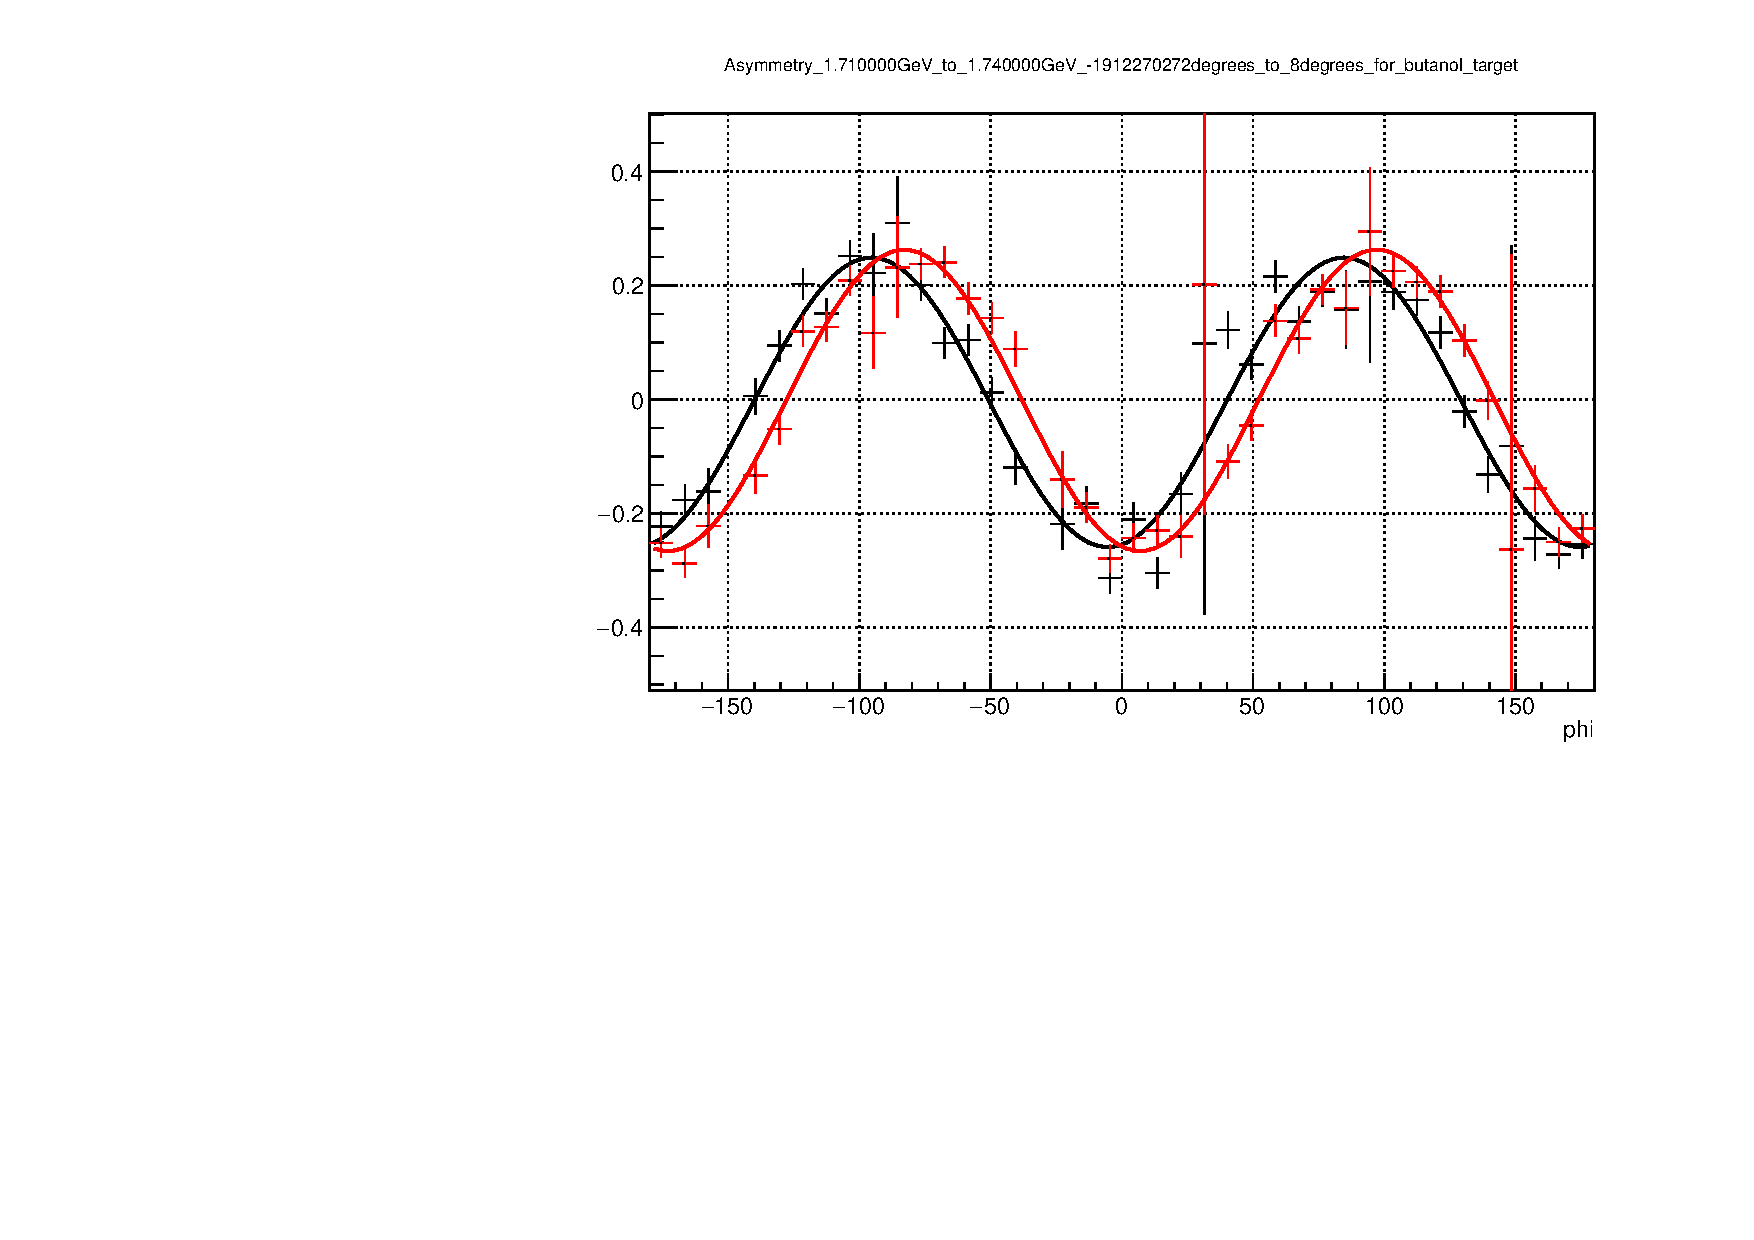
\includegraphics[width=0.9\textwidth]{figures/G_tgpol_effect.pdf} 
      \label{fig:GTgpol_theta1}
    }
    \caption{The Asymmetry histogram with the fit is plotted for the two different target polarization. One can see the simmetry of the shift from the nominal position in the center ($\phi = 0$).  One can see that, still after the weighting with the Amorphous flux, there is still some effect due to low statistics in the part separating the 6 sectors of CLAS}
    \label{fig:GTgpol}
  \end{center}
\end{figure} 
During the experimental data-taking PARA,PERP and AMO configurations were switched regularly. If data with the same configurations was taken at different periods (allowing a difference in $P_z$), the results were extracted separately (if statistically valuable). This allow us to safely consider for the target polarization
\begin{equation}
  (P_{+z\parallel}-P_{+z\perp}) \ll 1 \% 
\end{equation}
One can also use the harmonic mean ($\bar{p}$)for the PARA and PERP configurations of the photon polarization in order to further simplify equation \ref{eq:A1} 
\begin{equation}
  \frac{2}{\bar{p}} = \left(\frac{1}{P_{\gamma \parallel}} + \frac{1}{P_{\gamma \perp}}\right)
\end{equation}
Applying these two equations, one can obtain a simplified version for the created asimmetry
\begin{equation}
  \frac{N_{\parallel +} - N_{\perp +}}{N_{\parallel +} + N_{\perp +}} = \left( (\frac{1}{P_{\gamma \parallel}} - \frac{1}{P_{\gamma \perp}}) + 2 \Sigma cos(2(\phi-\phi_0)) +  (P_{+z\parallel}+P_{+z\perp}) G sin(2(\phi-\phi_0)) \right) \frac{\bar{p}}{2} \label{eq:A2}
\end{equation}
A fitted function was used in order to extract the values (after testing that $\phi_0$ was consistent with 0, the parameter was fixed in order to avoid extra fit fluctuations):
\begin{align}
  f(\phi) & = A + B cos(2(\phi-\phi_0)) + C sin(2(\phi-\phi_0)) \\
  \Sigma & = \frac{B}{D_F \, \bar{p}} \\
  G & = \frac{C}{D_F \, \bar{p} \,\bar{p_z}} \\
    \textnormal{where:} \, D_F & =   \textnormal{Dilution Factor} \\
    \bar{p_z} & =  \frac{P_{+z\parallel}+P_{+z\perp}}{2}
\end{align}
Results are obtained (See for example Fig. \ref{fig:GTgpol}) for both target polarizations (positive and negative) and are compared between each other (See appendix at \ref{app:G_TGPOL} and at \ref{app:Sigma_TGPOL}). Since both results looked part of the same statistical population, a weighted average of both measurements obtained from positive and negative target polarizations was used as conclusion. These results are presented in the next chapter.
